\paragraph{}
Comme nous l'avons expliqué dans la partie Réalisation, le diagramme de Gantt a dû être remanié au fil de l'avancement du projet car certaines tâches, plus faciles que prévues, ont été anticipées alors que d'autres, posant plus de problèmes, ont été allongées.
Le diagramme de Gantt final est donné page suivante et peut être comparé au diagramme fourni dans la [FIGURE].

\newpage
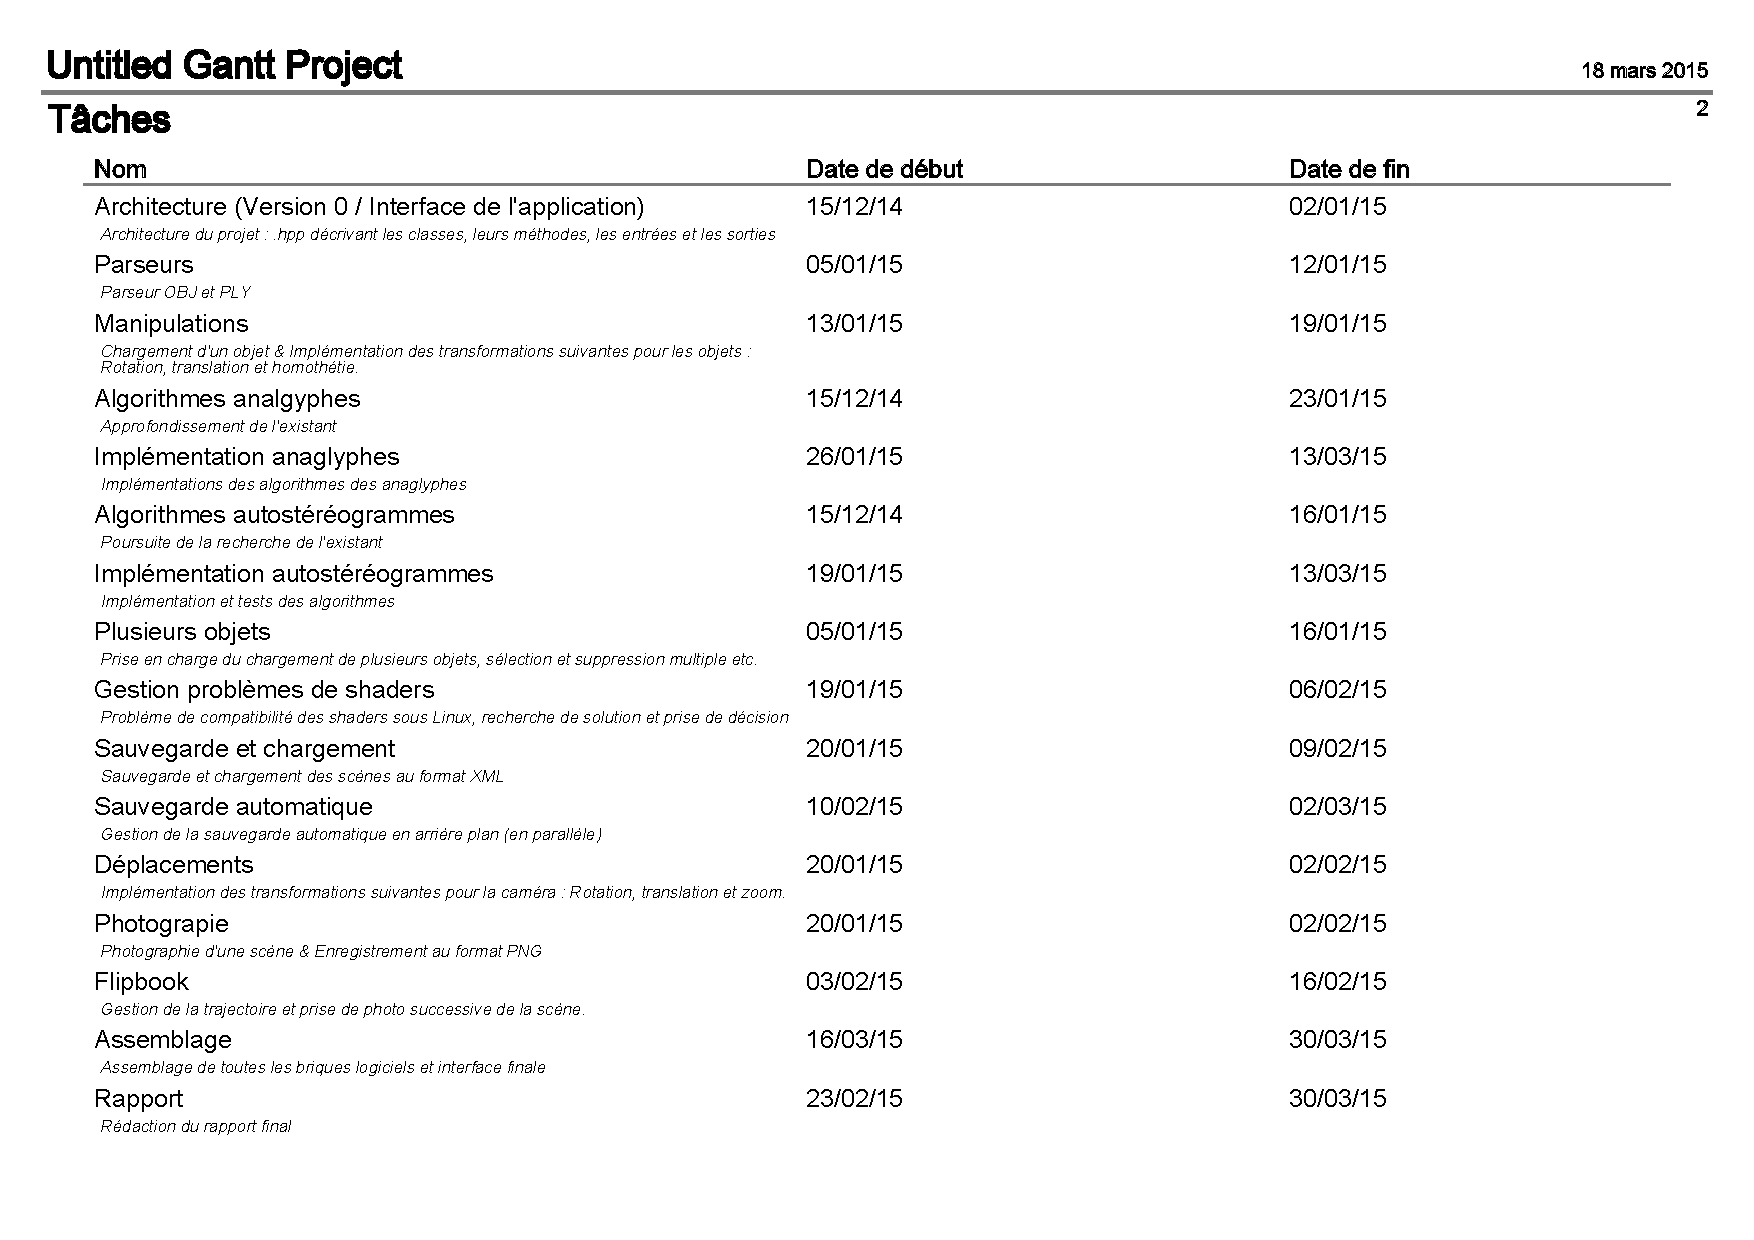
\includepdf[turn=false]{gantf.pdf}
\newpage

\paragraph{}
La principale modification consiste ainsi en l'allongement de la période destinée à la recherche d'algorithmes pour les rendus et à leur implémentation. Les raisons de cette différence ont été expliquées dans la partie Difficultés rencontrées ci-dessus.
Les manipulations des objets et de la scène ont été effectuées plus rapidement que prévu, mais une période de retour en arrière à cause des shaders a été ajoutée, allongeant la période de travail sur le chargement et la sauvegarde de la scène qui a été momentanément interrompue le temps de régler ce problème.

\paragraph{}
Malgré ces débordements dans le temps, la réalisation du projet se sera achevée dans les temps, le dernier mois ayant permis d'intégrer les algorithmes au logiciel, de compléter et de parfaire des fonctionnalités.
Au final, l'ensemble des manipulations de la scène et de ses objets qui avaient été promises dans le cahier des charges ont été implémentées. De même, l'ensemble des rendus prévu est générable à partir de la scène, et deux algorithmes de génération sont proposés pour les autostéréogrammes et les anaglyphes alors qu'un seul avait été cité pour l'autostéréogramme dans le cahier des charges, et que seul le traitement de couleurs pour l'impression avait été initialement prévu pour m'anaglyphe (et pas la saturation).

\paragraph{}
Au niveau des besoins non fonctionnels, la portabilité aura été respectée malgré l'utilisation des shaders qui auraient pu poser problème sur certaines machines. Grâce aux nombreux modules proposés par la bibliothèque Qt, portable et très complète, des solutions auront été trouvées pour l'ensemble des modules et des cas d'utilisation sans avoir à sacrifier de fonctionnalité pour permettre l'utilisation du logiciel aussi bien sous Windows que sous Linux.

\paragraph{}
Bien que l'indication ne soit pas donnée dans le logiciel, l'utilisation de [NOM DU LOGICIEL] en parallèle de l'utilisation du logiciel nous a permis de vérifier la fluidité du logiciel. Grâce notamment au modèle 'happy.ply' présenté dans le cahier des charges, les valeurs de frames par seconde données dans le cahier des charges ont été validées.
[Redonner les valeurs]
[Vérifier sur plusieurs machines]

\paragraph{}
Enfin, la maintenabilité du logiciel sera également possible grâce au choix des outils et à l'architecture du projet. 
Tout d'abord, l'utilisation de Qt5, qui est actuellement la plus récente de Qt, laisse envisager que le logiciel pourra être utilisé longtemps sans avoir à migrer vers une nouvelle version de la bibliothèque. Ensuite, l'utilisation de OpenGL ES 2.0, qui est la version d'OpenGL de base avec Qt5, pourrait éventuellement permettre de générer une application mobile du logiciel. 
L'architecture a également été pensée pour permettre cette maintenabilité. En effet, comme le prouvent les deux algorithmes 


\paragraph{}
Ce bilan positif montre que l'ensemble des besoins fonctionnels et non fonctionnels ciblés dans le cahier des charges ont été implémentés avec succès. Nous espérons que ce projet sera réutilisé et maintenu, puisqu'il a été conçu dans cet optique. Il sera éventuellement possible de générer une application mobile à partir du code existant, ou d'ajouter et de tester d'autres algorithmes ou d'autre rendus possible à partir d'une scène en trois dimensions. Nous espérons également que nos clients auront été satisfaits du travail réalisé et du logiciel final. 
